\documentclass[a4paper,fontset = windowsnew]{ctexbook}
\usepackage{xifthen}
\usepackage{calc}
\usepackage{graphicx}
\usepackage{tikz}
%\usepackage{amsmath}
\usepackage{cexam}

\begin{document}
\chapter{基本排版程序}

\ExplSyntaxOn

\parindent=0pt

%%%%模块测试

\rule{\linewidth}{1pt}\newline
这是参考文本
这是参考文本
这是参考文本
这是参考文本
这是参考文本
这是参考文本
这是参考文本
这是参考文本
这是参考文本
这是参考文本
这是参考文本
这是参考文本
这是参考文本
这是参考文本
%\int_set:Nn \cexam_number_int {100}
\par
\selection_type:n 
1.高中物理中电场和磁场是相当重要的一部分内容,
<:
%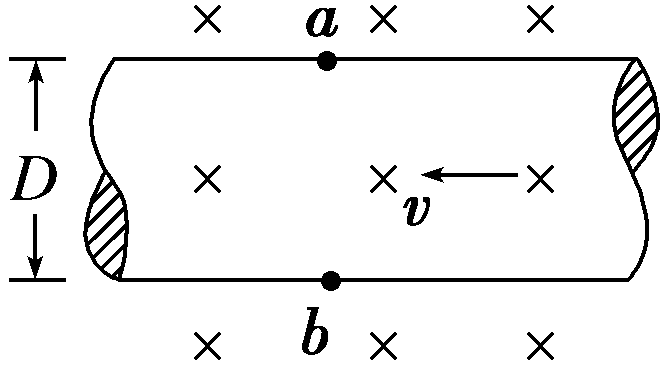
\includegraphics{1.png}
\begin{tikzpicture}
  \draw (0,0) rectangle (3,5);
\end{tikzpicture}
:>
所示是常见的一种情况.横向电压为
\begin{equation}
  E=MC^2
\end{equation}
请选出正确的答案
\begin{equation}
  E=MC^2
\end{equation}
请选出正确的答案
A.这是
B.这是
C.这是
D.这是
\scan_stop:


\end{document}
